\documentclass[10pt,a4paper]{article}
\usepackage[english]{babel}
\usepackage[utf8]{inputenc}
\usepackage[T1]{fontenc}
\usepackage{lmodern,microtype}
\usepackage[a4paper,top=2.4cm,bottom=2.3cm,left=2.65cm,right=2.65cm]{geometry}
\usepackage{amsmath,graphicx,float,booktabs}
\usepackage{xcolor}
\usepackage[font=small,labelfont=bf]{caption}
\usepackage[hidelinks]{hyperref}
\hypersetup{pdftitle={From Random Windows to Future Forecasts},
  pdfsubject={A replication of DeLELSTM on three forecasting benchmarks}}
\setlength{\intextsep}{9pt plus 2pt minus 2pt}
\setlength{\parindent}{1.15em}
\raggedbottom

\begin{document}
\begin{center}
  {\fontsize{30}{33}\selectfont\bfseries
   From Random Windows\\
   to Future Forecasts\par}
  \vspace{7pt}
  {\sffamily\fontsize{13}{16}\selectfont\color[HTML]{42454A}
   A Replication of DeLELSTM on Three Forecasting Benchmarks\par}
  \vspace{8pt}
  {\color[HTML]{AA2156}\rule{32pt}{1.1pt}\par}
  \vspace{7pt}
  {\small
   \begin{tabular}{@{}c@{\hspace{1.8em}}c@{\hspace{1.8em}}c@{}}
     CHEN Canyang & GUAN Wenxi & DONG Zhangyan \\[2pt]
     XING Zhixuan & XU Rufei & ZHUANG Erdong
   \end{tabular}\par}
  \vspace{5pt}
  {\small\sffamily\color[HTML]{42454A}
   DSC6013\,\textperiodcentered\, Group 17\,\textperiodcentered\, Option A\par}
\end{center}

\begin{abstract}
How closely does a published exchange-rate error describe a forecast made one day ahead? When rolling windows are randomly split, the same dates can appear in training and testing. We used this distinction to revisit DeLELSTM, a recurrent model that assigns separate weights to a variable's history and its latest change. Across 75 training runs, we recovered the published winner by mean root mean squared error (RMSE) on each of three datasets. All three replicated DeLELSTM means were within 1.2\% of the published values. Yet every one of the 757 random Exchange test windows shared a source day with training. We therefore evaluated DeLELSTM on three successive periods per dataset, with training-only scaling and no shared source times across partitions. Relative to the complete random-test reference, mean RMSE was lower in all three PM2.5 periods, higher in all three Exchange periods and mixed for Electricity. Recovering the benchmark winners and measuring forecast accuracy on later dates required two different experiments.
\end{abstract}

\section{Introduction}
Suppose a model predicts the next Singapore exchange rate from the previous month's rates. A 30-day window starting on Monday and another starting on Tuesday share 29 observations. If one window enters training and the other enters testing, the model can score well on held-out windows that contain familiar dates. A reader interested in the next trading day needs to know which observations were available when the model was fitted.

DeLELSTM is a useful case because its forecasts come with an account of how the model used each variable. Wang et al.~\cite{wang} separate the hidden state carried from the previous step from its latest change and fit weights to both. Their reported results invite two questions. Can we reproduce the forecast errors and recover an interpretable pattern from the fitted weights? How well does the model predict a period that begins after training and validation have ended?

We first repeated the authors' five-model comparison on electricity consumption, air pollution and exchange rates. We then held the fitted weights fixed and restored the omitted test windows, isolating the effect of scoring coverage. Finally, we traced the underlying dates, trained DeLELSTM on successively longer histories and scored it on the next test period. The first comparison measures variation across training runs, the second tests sensitivity to which windows count, and the third measures performance on a later period.

\section{Forecasting task and model}\label{sec:model}
Each prediction is one step ahead. Electricity uses hourly consumption and 15 weather variables, PM2.5 uses hourly Beijing pollution and meteorological observations, and Exchange uses eight daily rates to predict the Singapore rate. Electricity and PM2.5 group 24 hours into a daily window. Exchange advances a 30-day window by one observation at a time. After an initial step, the released model produces 22 hourly or 28 daily predictions per window, updating its inputs at each step.

\newpage
At step \(t\), a standard LSTM produces a shared state \(H_t\) from all variables. A second, tensorized LSTM updates a separate state \(h_t^d\) for each variable \(d\). To reconstruct the shared state, the model fits a weight to the previous state of each variable and another to the change since that step. Their weighted sum gives the reconstructed state
\[
  \widehat H_t = \sum_{d=1}^D
    \bigl(\alpha_t^d h_{t-1}^d + \beta_t^d (h_t^d-h_{t-1}^d)\bigr)
  \;\approx\; H_t .
\]
The columns of the design matrix \(A_t\) are these \(2D\) vectors. For each window and step, the code solves the unregularized normal equations, using the pseudoinverse of \(A_t^\top A_t\) if its inverse fails. A linear readout of \(\widehat H_t\) gives the next prediction. The standard branch also receives \(\widehat H_t\) at its next step. This construction makes the fitted coefficients available alongside each forecast.

\section{What the published benchmark reproduces}\label{sec:replication}
\subsection{The published RMSE winners recur on all three datasets}
We compared DeLELSTM with LSTM~\cite{lstm}, RETAIN~\cite{retain}, IMV-Full and IMV-Tensor~\cite{imv} using the released evaluation. Inputs were min--max scaled over the full series before windows were randomly allocated to training (75\%), validation (15\%) and testing (about 10\%). With the split seed fixed at 555, five training repetitions for each model and dataset yielded 75 results. Training used Adam~\cite{adam}, mean squared error, a validation-based learning-rate schedule and best-validation checkpoint selection. Batch sizes were 64/32/128 and training lasted 350/300/300 epochs for Electricity/PM2.5/Exchange, respectively. These runs used a macOS CPU, Python 3.13 and PyTorch 2.10.0.

DeLELSTM had the lowest mean RMSE on Electricity and Exchange. RETAIN had the lowest mean on PM2.5. The same three winners appear in the published table. On PM2.5, where the DeLELSTM mean differed most in relative terms, it was 26.3124 here and 26.612 in the paper (Table~\ref{tab:1}). LSTM and DeLELSTM exchanged places on PM2.5, where their mean errors were close in both studies.

\begin{table}[H]
\centering
\caption{Test RMSE on the released random-window benchmark. Replication values are means and sample standard deviations over five training repetitions on a fixed split. Bold marks the lowest mean within each dataset. The last column gives the published means at their reported precision~\cite{wang}. RMSE is in the target's original units.}\label{tab:1}
\small
\begin{tabular}{@{}llrr@{}}
\toprule
\textbf{Dataset} & \textbf{Model} & \textbf{Replication (mean \(\pm\) SD)} & \textbf{Published mean} \\
\midrule
Electricity & DeLELSTM & \textbf{1.7185} \(\pm\) 0.0596 & \textbf{1.7247} \\
 & IMV-Full & 1.9995 \(\pm\) 0.0751 & 2.0284 \\
 & IMV-Tensor & 2.3636 \(\pm\) 0.1947 & 2.6069 \\
 & LSTM & 5.1152 \(\pm\) 6.9259 & 5.1049 \\
 & RETAIN & 2.6980 \(\pm\) 0.2287 & 2.6685 \\
\addlinespace PM2.5 & DeLELSTM & 26.3124 \(\pm\) 0.4471 & 26.612 \\
 & IMV-Full & 28.6004 \(\pm\) 0.6386 & 28.465 \\
 & IMV-Tensor & 29.3094 \(\pm\) 0.9821 & 28.866 \\
 & LSTM & 26.5177 \(\pm\) 0.1724 & 26.566 \\
 & RETAIN & \textbf{24.9538} \(\pm\) 0.0536 & \textbf{24.913} \\
\addlinespace Exchange & DeLELSTM & \textbf{0.002293} \(\pm\) 0.000069 & \textbf{0.0023} \\
 & IMV-Full & 0.002626 \(\pm\) 0.000011 & 0.0026 \\
 & IMV-Tensor & 0.002638 \(\pm\) 0.000004 & 0.0026 \\
 & LSTM & 0.002619 \(\pm\) 0.000005 & 0.0026 \\
 & RETAIN & 0.002485 \(\pm\) 0.000020 & 0.0025 \\
\bottomrule
\end{tabular}
\end{table}

\begin{figure}[H]
\centering
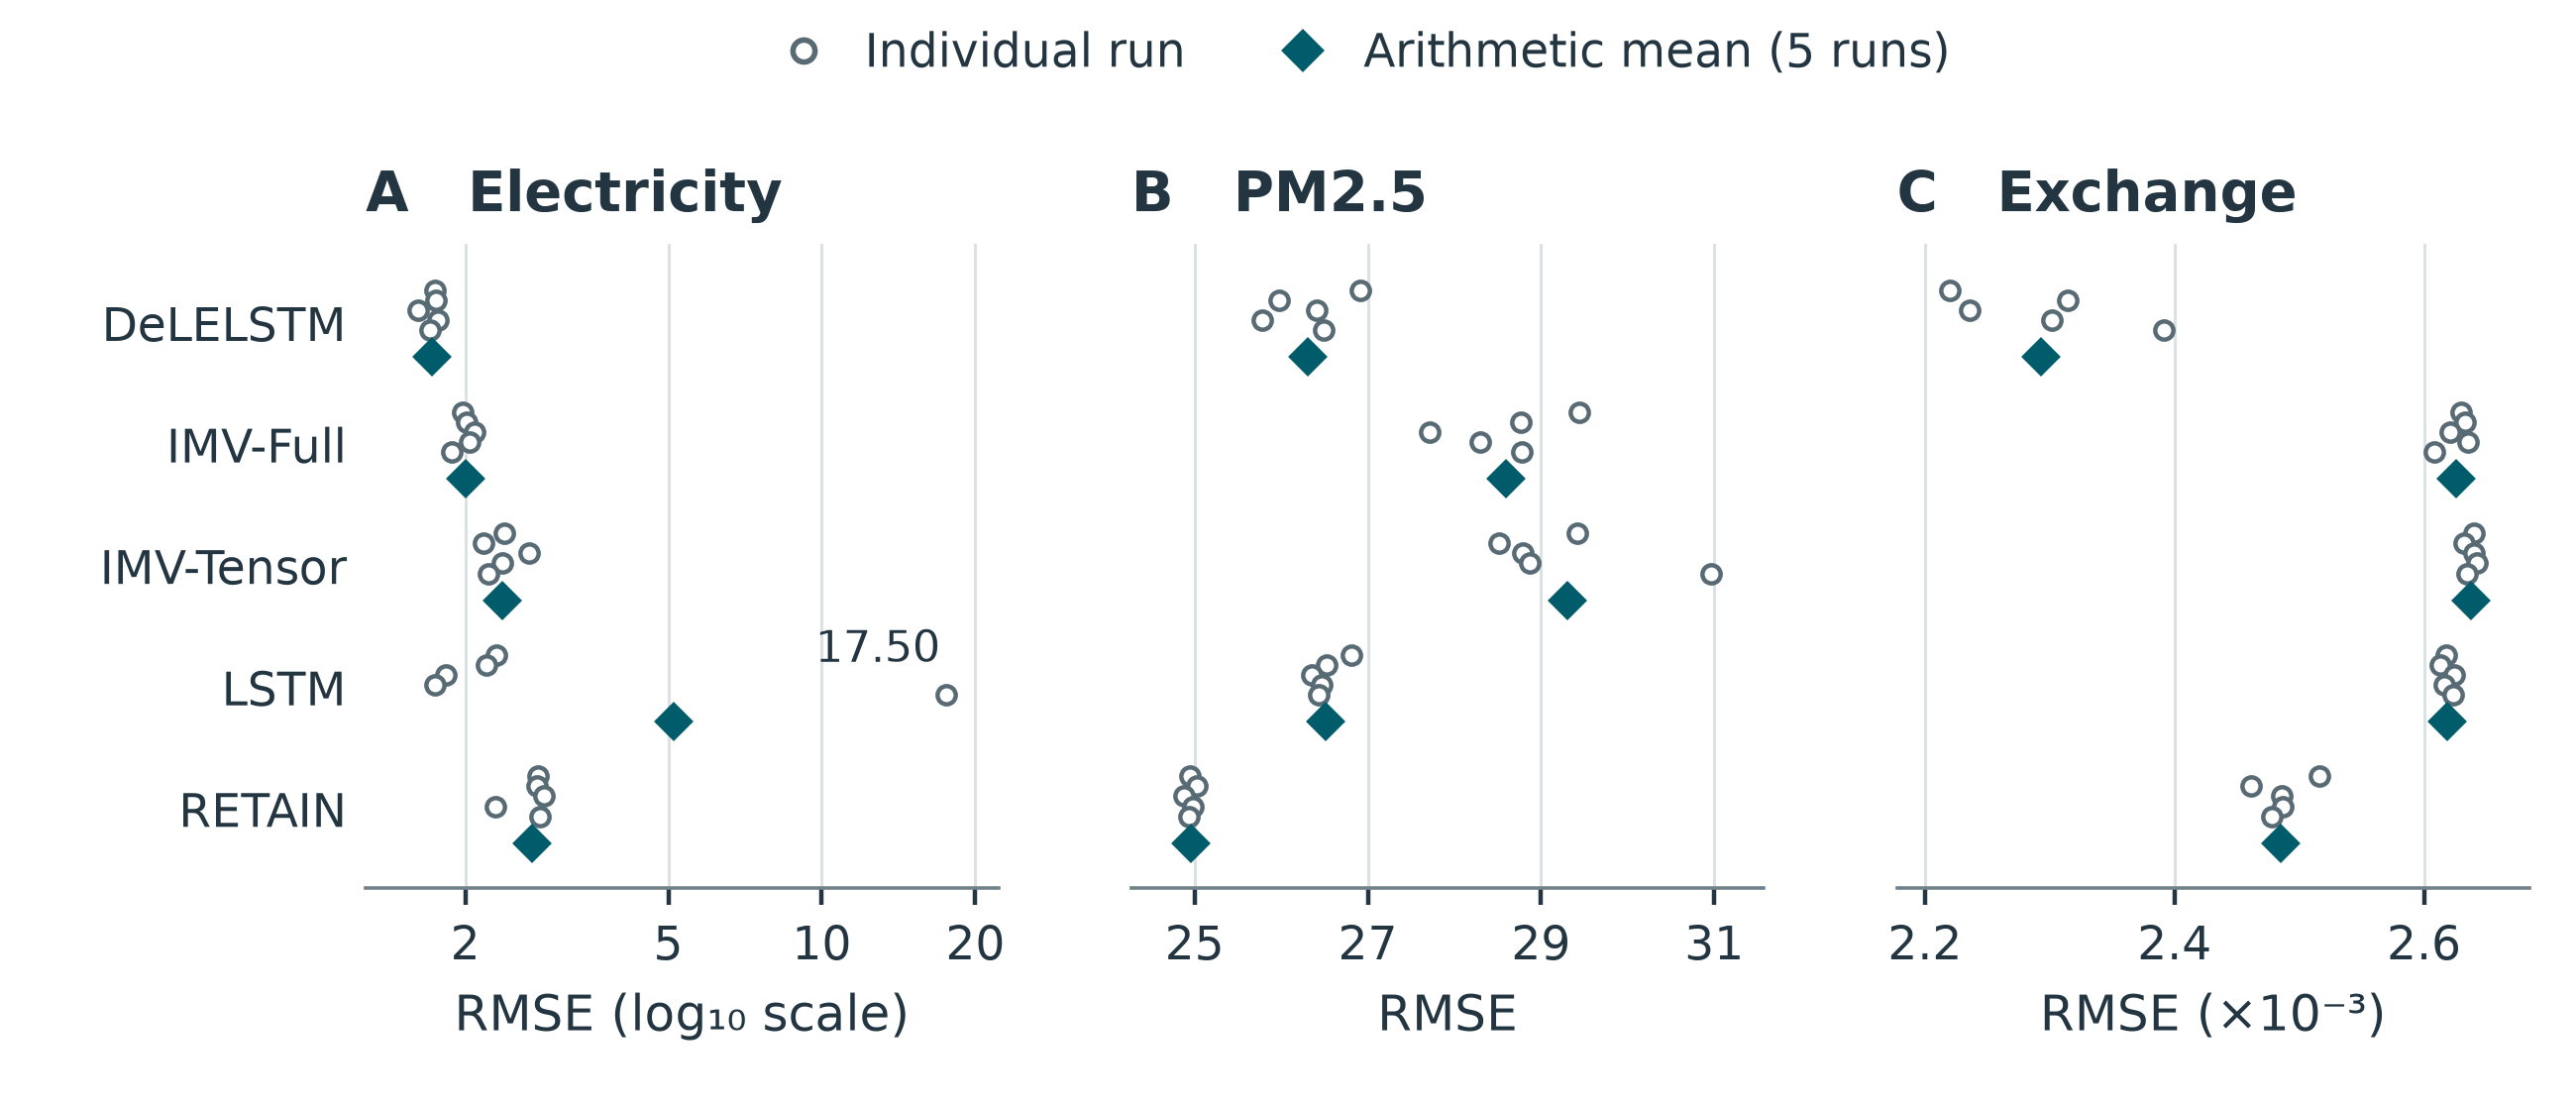
\includegraphics[width=0.98\linewidth]{figure_1.png}
\caption{Individual runs (circles) and their arithmetic means (diamonds) on the fixed random split. Electricity uses a logarithmic axis to accommodate the LSTM run at 17.50. Exchange tick labels are in units of \(10^{-3}\).}\label{fig:1}
\end{figure}

Figure~\ref{fig:1} shows why individual runs matter for interpreting the means. Four Electricity LSTM runs had RMSE between 1.74 and 2.31. The fifth reached 17.50, bringing the mean to 5.12. The published table likewise reports a large standard deviation for this model (6.37). Since all five repetitions share a split, their spread measures training variability on those particular windows. The historical PM2.5 campaign used seeds 556--560 after an earlier seed-555 initialization failed. Its summary describes completed runs.

\subsection{The PM2.5 history coefficient gains share between the first and last outputs}
For the PM2.5 input itself, we asked how its balance of history and change evolved as the model read through the day. For each checkpoint and output position we used the released coefficients averaged over retained test windows. We took absolute values and normalized the historical and change coefficients separately across variables (L1), giving \(\tilde\alpha_t^d\) and \(\tilde\beta_t^d\). The instantaneous share
\(I_t^d=\tilde\beta_t^d/(\tilde\alpha_t^d+\tilde\beta_t^d)\)
measures the balance for a given variable. The corresponding global importance, \(T^{-1}\sum_t\sqrt{(\tilde\alpha_t^d)^2+(\tilde\beta_t^d)^2}\), measures its overall coefficient magnitude. A large share can occur even when both coefficients are small.

Across five runs, the mean instantaneous share for PM2.5 was \(0.603\pm0.183\) at the first output and \(0.023\pm0.022\) at the last. All five ended below their own starting value (Figure~\ref{fig:2}). At the final update the coefficient balance favored the variable's accumulated history, while the first update varied considerably across runs. This is a statement about fitted weights at positions within a window. Every daily window starts at midnight, so clock hour and position within the window coincide. The profiles average across days and cannot distinguish either effect from the other or identify the physical causes of pollution.

\begin{figure}[H]
\centering
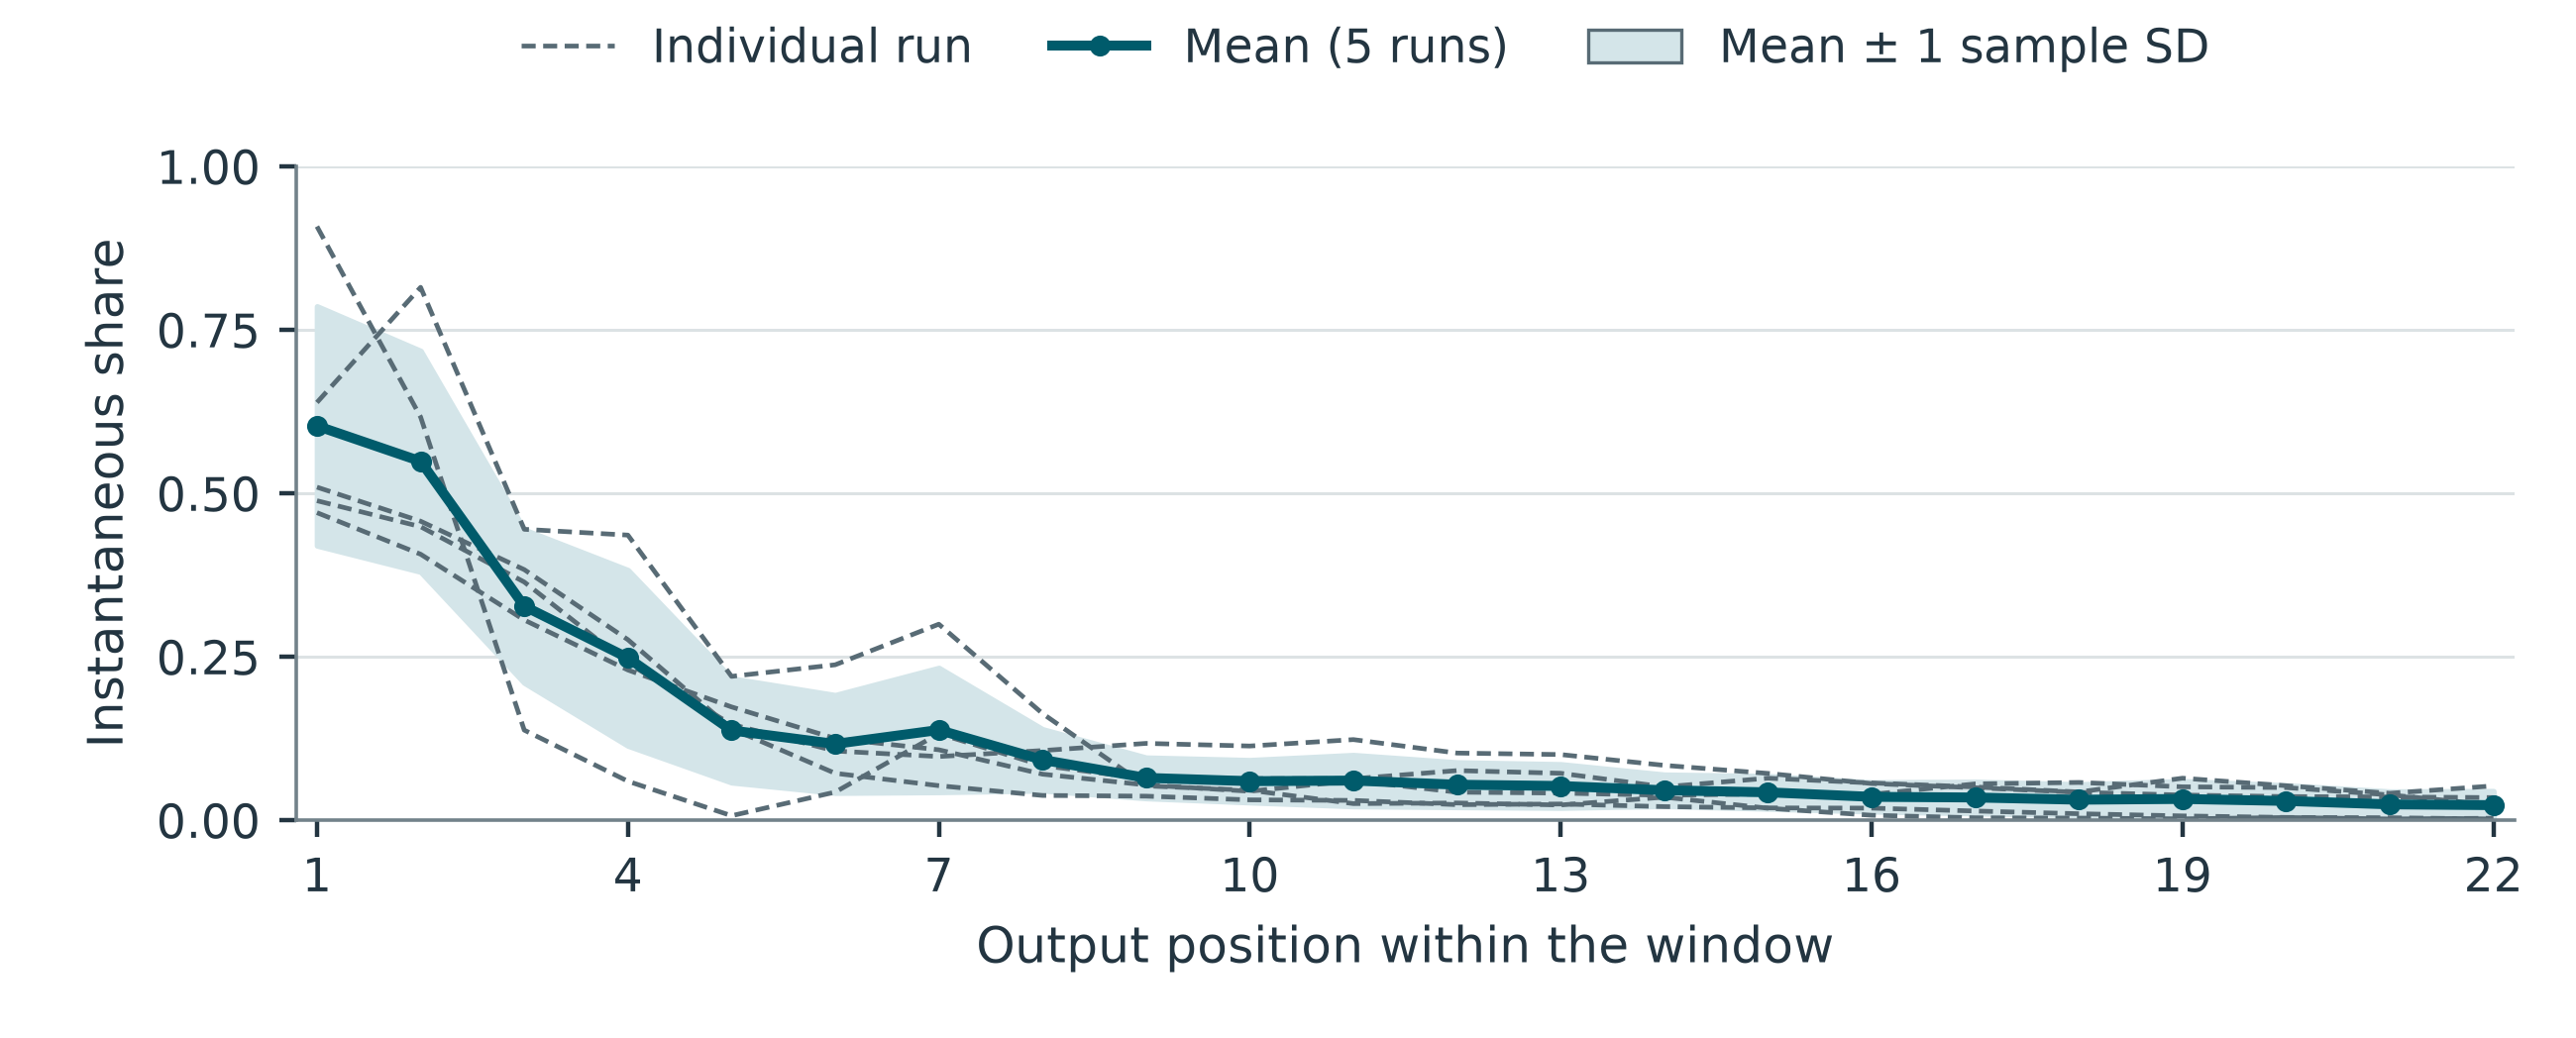
\includegraphics[width=0.82\linewidth]{figure_2.png}
\caption{PM2.5's instantaneous share at 22 successive one-hour-ahead outputs within the daily window. Dashed lines show the five runs. The solid line is their mean and the band spans one sample SD, clipped to \([0,1]\).}\label{fig:2}
\end{figure}

\section{Which observations entered the benchmark?}\label{sec:audit}
\subsection{Restoring every test window gives a common reference}\label{sec:attrition}
The released validation and test loaders discard the final incomplete batch. The benchmark therefore scored 64 of 92 Electricity windows, 160 of 184 PM2.5 windows and 640 of 757 Exchange windows. We rescored the same 15 DeLELSTM checkpoints twice, first reproducing the saved score on retained windows and then including the final batch. No weights changed. Mean RMSE moved from 1.7185 to 1.6825 on Electricity, from 26.3124 to 25.6103 on PM2.5 and from 0.002293 to 0.002273 on Exchange. Error fell in 14 of the 15 pairs (Figure~\ref{fig:3}). These complete-test means provide the historical reference for the later periods. Appendix~\ref{app:records} gives the across-run standard deviations. Checkpoint selection still used the original validation loader.

\begin{figure}[H]
\centering
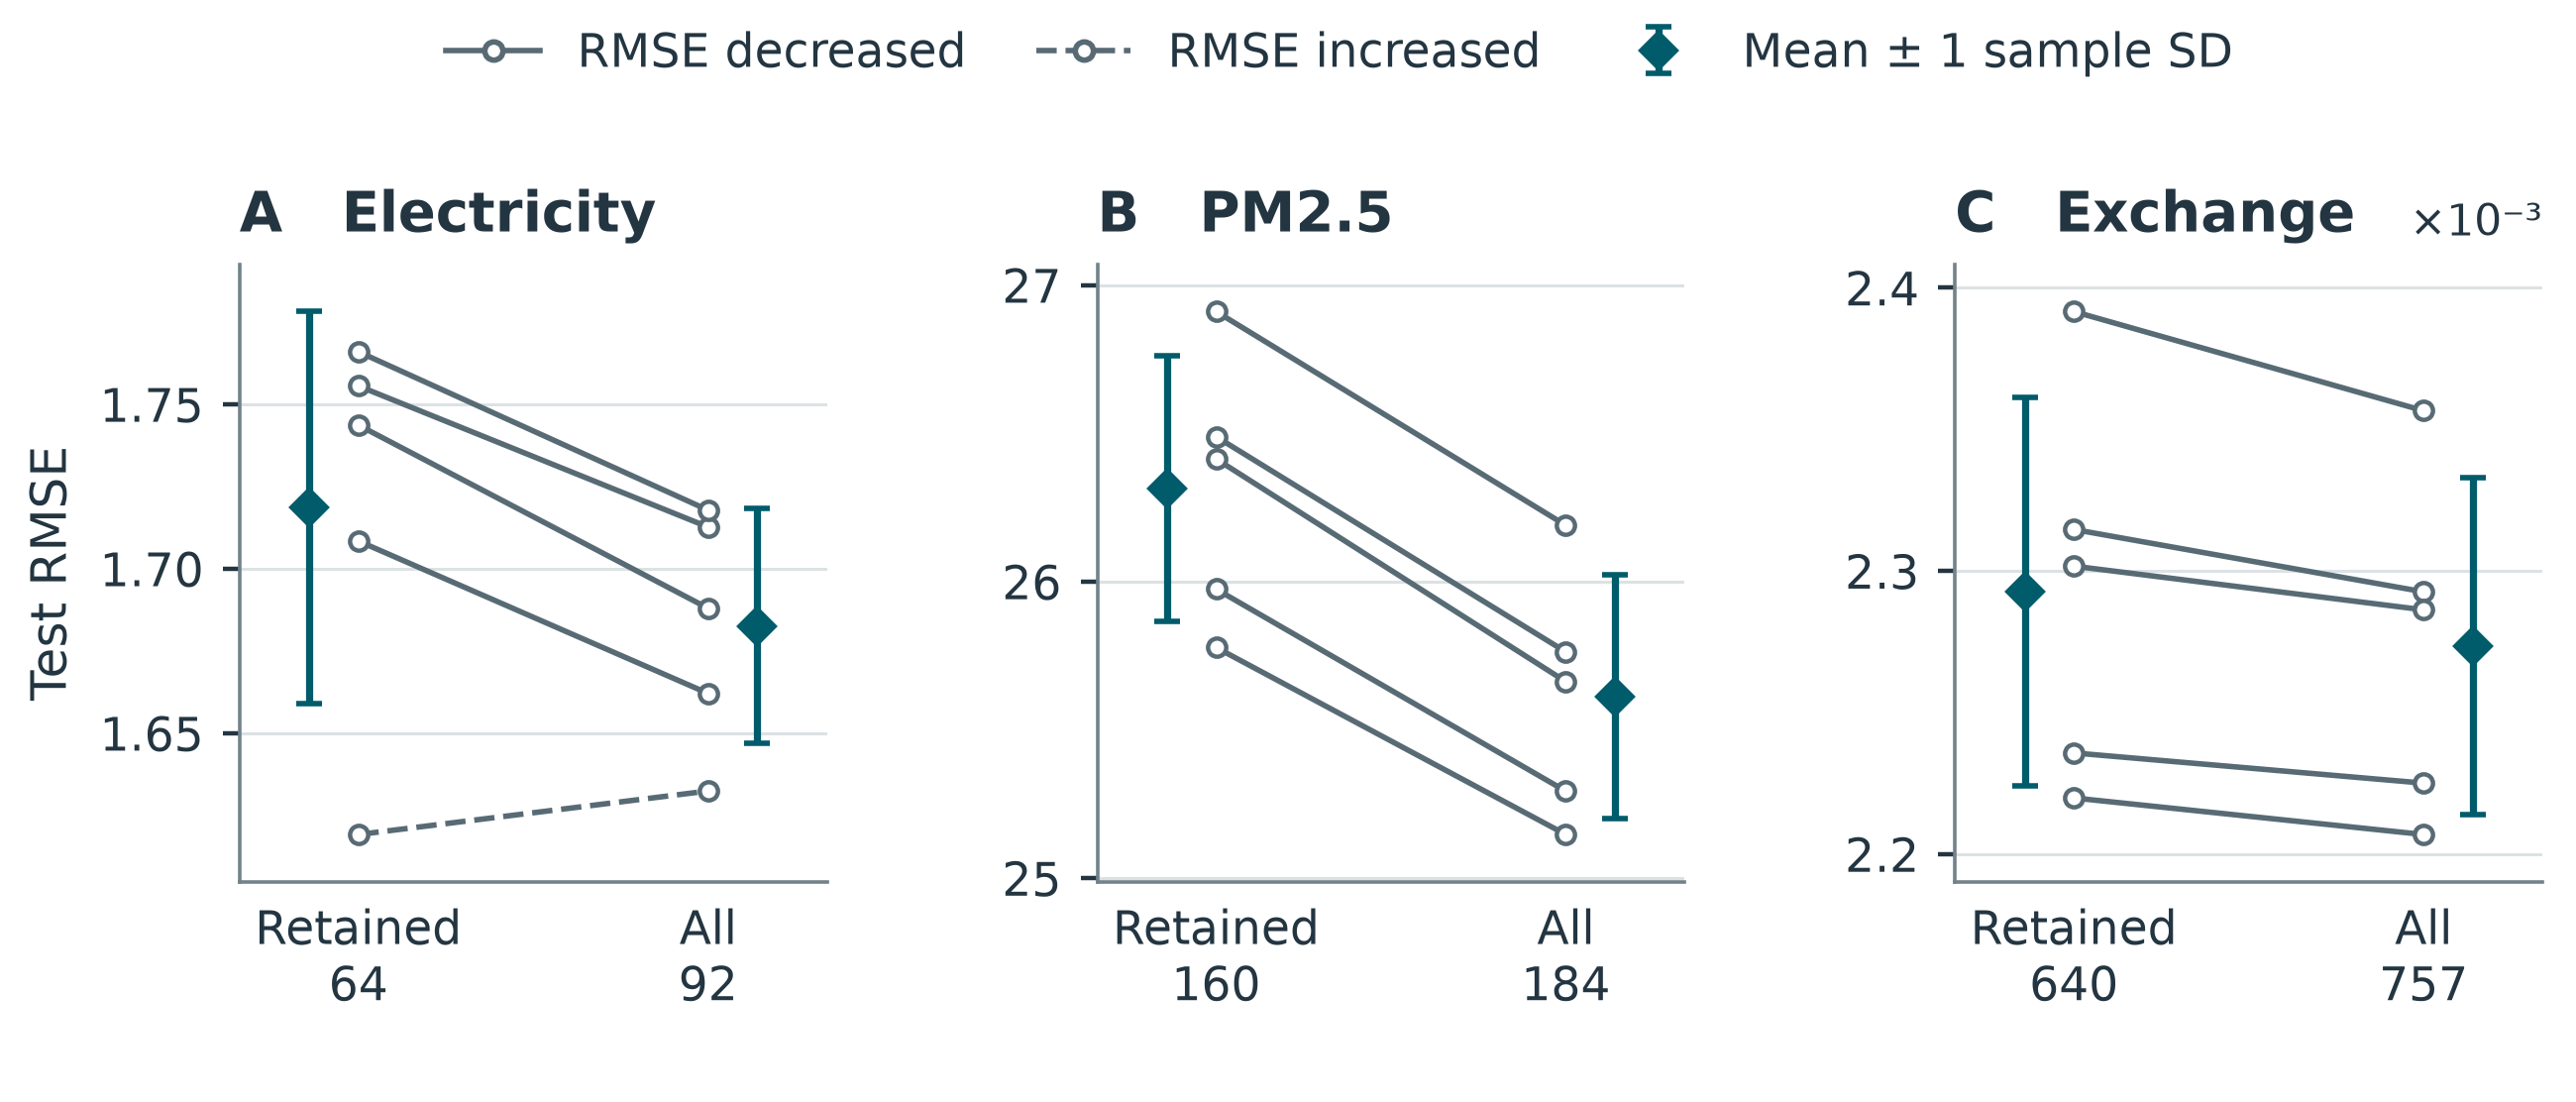
\includegraphics[width=0.93\linewidth]{figure_3.png}
\caption{Test RMSE for retained and complete batches at fixed weights. A line joins two evaluations of one checkpoint. The dashed Electricity line marks the one increase. Diamonds and whiskers show five-run means and one sample SD. Panel scales differ.}\label{fig:3}
\end{figure}

\subsection{Holding out a window can leave its dates in training}
Restoring the final batch tells us which windows counted. Tracing their dates reveals what the fit could already have seen. On Exchange, \emph{all 757} random test windows shared at least one source day with a training window. For 713 of them a training window began just one day away. The original hourly datasets used non-overlapping days, but random assignment still placed some training days after test days in both series.

Held-out observations also affected scaling. In the random PM2.5 training windows, the pollutant input ranged from 1 to 886. The released scaler used 0 and 994, the extrema across the full series. Thus even an observation well inside the training period received a value that depended on data assigned to validation or testing.

\section{Forecasting the next held-out period}\label{sec:chronology}
\subsection{What was available at forecast time?}
For each dataset we ordered windows by source time and formed three expanding training sets covering the first 55\%, 65\% and 75\% of starts. Each training set was followed by a 15\% validation period and a 10\% test period. We fixed the boundaries first. For Exchange, we then removed the first 29 window starts from the later partition at each boundary. Across all nine dataset--fold combinations, training, validation and testing shared zero source time points within a fold.

For each feature we fitted the minimum and maximum on retained training windows and reused them without clipping on later inputs. Perturbing the held-out inputs left scaled training values unchanged. For PM2.5 the original preprocessing filled the first 24 missing hours with the first subsequent reading of 129. We rebuilt inputs by carrying observations forward and excluded the first day, which had no prior reading. Only observed targets entered the training loss, validation score and test metrics. In the final test period, 3,964 of 4,026 forecast positions had observed targets (Table~\ref{tab:2}).

\begin{table}[H]
\centering
\caption{Coverage in the final chronological fold, after boundary exclusions. The last column counts scored forecast positions and all candidate positions. Exchange is indexed by source row.}\label{tab:2}
\small
\begin{tabular}{@{}lrrrlr@{}}
\toprule
\textbf{Dataset} & \shortstack[r]{\textbf{Train}\\\textbf{windows}} & \shortstack[r]{\textbf{Val.}\\\textbf{windows}} & \shortstack[r]{\textbf{Test}\\\textbf{windows}} & \textbf{Test period} & \shortstack[r]{\textbf{Scored / total}\\\textbf{test targets}} \\
\midrule
Electricity & 686 & 137 & 92 & 25 Mar--24 Jun 2020 & 2,024 / 2,024 \\
PM2.5 & 1,368 & 274 & 183 & 2 Jul--31 Dec 2014 & 3,964 / 4,026 \\
Exchange & 5,669 & 1,105 & 727 & Rows 6,832--7,587 & 20,356 / 20,356 \\
\bottomrule
\end{tabular}
\end{table}

\subsection{The same architecture across three future periods}\label{sec:forecasts}
We trained DeLELSTM for each fold on one H100 (PyTorch 2.7.1, CUDA 12.6), with the original epoch counts and batch sizes. Each checkpoint was selected on the full validation partition and scored on every test window in the subsequent period. Electricity and Exchange used seeds 555--559 and PM2.5 used 556--560.

\begin{table}[H]
\centering
\caption{DeLELSTM test RMSE on successive future periods. Means and sample SDs are across successful seeds. Targets count scored positions per run. In PM2.5 fold 2, seed 556 stopped with non-finite loss and seed 559 with a non-finite gradient.}\label{tab:3}
\small
\begin{tabular}{@{}lrlrrr@{}}
\toprule
\textbf{Dataset} & \textbf{Fold} & \textbf{Test interval} & \shortstack[r]{\textbf{Scored}\\\textbf{targets}} & \shortstack[r]{\textbf{Seeds}\\\textbf{succeeded}} & \shortstack[r]{\textbf{Test RMSE}\\\textbf{Mean \(\pm\) sample SD}} \\
\midrule
Electricity & 1 & 22 Sep--22 Dec 2019 & 2,024 & 5/5 & 1.6299 \(\pm\) 0.0682 \\
Electricity & 2 & 23 Dec 2019--24 Mar 2020 & 2,002 & 5/5 & 1.5753 \(\pm\) 0.0613 \\
Electricity & 3 & 25 Mar--24 Jun 2020 & 2,024 & 5/5 & 1.9677 \(\pm\) 0.0236 \\
PM2.5 & 1 & 2 Jul--30 Dec 2013 & 3,961 & 5/5 & 18.09 \(\pm\) 0.24 \\
PM2.5 & 2 & 31 Dec 2013--1 Jul 2014 & 3,999 & 3/5 & 23.01 \(\pm\) 0.32 \\
PM2.5 & 3 & 2 Jul--31 Dec 2014 & 3,964 & 5/5 & 17.85 \(\pm\) 0.05 \\
Exchange & 1 & Rows 5,320--6,075 & 20,356 & 5/5 & 0.025994 \(\pm\) 0.007192 \\
Exchange & 2 & Rows 6,076--6,831 & 20,356 & 5/5 & 0.008203 \(\pm\) 0.003832 \\
Exchange & 3 & Rows 6,832--7,587 & 20,356 & 5/5 & 0.005136 \(\pm\) 0.001467 \\
\bottomrule
\end{tabular}
\end{table}

Relative to the complete random-test reference, PM2.5 had lower mean RMSE in every period (17.85--23.01 versus 25.6103). Electricity fell below its reference of 1.6825 twice and rose above it in the last period. Exchange remained above 0.002273 in all three periods, including the last, when mean RMSE was 0.005136. Table~\ref{tab:3} gives all nine results. The middle PM2.5 mean uses three successful seeds. Overall, 43 of the 45 planned runs produced a test score.

\section{Discussion and conclusion}
The benchmark replication answers a question about model comparison. DeLELSTM and RETAIN led on exactly the datasets where the original paper placed them first by mean RMSE. Across all five PM2.5 checkpoints, the historical coefficient also took a larger share at the last output than at the first. Testing whether the most highly ranked variables suffice for prediction would require the pending five-seed variable-selection experiment.

The chronological evaluation answers a question about forecasting. For the Singapore rate, every random test window shared observations with training. Removing cross-partition overlap gave us three periods in which the fitted model had seen none of the test dates. PM2.5 and Exchange fell on opposite sides of their random-test references, and Electricity changed sides across periods. Which observations enter the score matters even when the architecture stays fixed.

Only DeLELSTM was trained on the chronological folds. Between protocols, the training histories, test observations and computing environments changed, and the random PM2.5 reference included filled targets. Isolating the effect of any one preprocessing choice would require holding the future test windows, observed targets and seeds fixed while varying that choice. The practical result of this replication is a way to read each forecast error alongside the dates used to fit the model, the windows actually scored and the observations available at the time of prediction.

\appendix
\section{Inference cost and supplementary metrics}\label{app:metrics}
\subsection{Inference on one H100}
We timed the lowest scheduled seed in the last fold for each dataset on an NVIDIA H100 80\,GB HBM3. Timing used FP32 with TF32 disabled and included the coefficient solves. Inputs and weights were already on the device. After ten warm-up calls, we timed each single window with GPU synchronization. Batched throughput covered ten passes through the full test set after one warm-up pass. At the stated batch sizes, predictions matched the archived values at every output position.

\begin{table}[H]
\centering
\caption{Single-window latency and batched throughput in the final fold. P50 denotes the median, P95 the 95th percentile.}\label{tab:4}
\small
\begin{tabular}{@{}lrrrrr@{}}
\toprule
\textbf{Dataset} & \textbf{Test windows} & \textbf{P50 (ms)} & \textbf{P95 (ms)} & \textbf{Batch size} & \textbf{Throughput (windows/s)} \\
\midrule
Electricity & 92 & 18.50 & 22.49 & 64 & 2,155 \\
PM2.5 & 183 & 17.07 & 17.49 & 32 & 1,697 \\
Exchange & 727 & 18.99 & 22.06 & 128 & 5,317 \\
\bottomrule
\end{tabular}
\end{table}

\subsection{Fixed-split MAE and MAPE}
Table~\ref{tab:additional} gives the other two reported accuracy metrics. MAE uses the target's original scale, and MAPE is expressed as a percentage. Each cell is the mean and sample SD across the same five completed historical runs used in Table~\ref{tab:1}.
\begin{table}[H]
\centering
\caption{Complete fixed-split results for mean absolute error and mean absolute percentage error.}\label{tab:additional}
\small
\begin{tabular}{@{}llrr@{}}
\toprule
\textbf{Dataset} & \textbf{Model} & \textbf{MAE} & \textbf{MAPE (\%)} \\
\midrule
Electricity & DeLELSTM & 1.0995 \(\pm\) 0.0237 & 1.6885 \(\pm\) 0.0422 \\
 & IMV-Full & 1.3570 \(\pm\) 0.0913 & 2.1592 \(\pm\) 0.1784 \\
 & IMV-Tensor & 1.6627 \(\pm\) 0.1835 & 2.6858 \(\pm\) 0.3368 \\
 & LSTM & 3.9564 \(\pm\) 5.8129 & 6.4844 \(\pm\) 9.6383 \\
 & RETAIN & 2.0365 \(\pm\) 0.2012 & 3.2644 \(\pm\) 0.3215 \\
\addlinespace
PM2.5 & DeLELSTM & 13.4022 \(\pm\) 0.1497 & 22.0590 \(\pm\) 1.2380 \\
 & IMV-Full & 14.1497 \(\pm\) 0.4155 & 23.7698 \(\pm\) 0.8981 \\
 & IMV-Tensor & 14.7603 \(\pm\) 0.8001 & 27.5900 \(\pm\) 2.9759 \\
 & LSTM & 13.4993 \(\pm\) 0.1734 & 22.3953 \(\pm\) 1.3112 \\
 & RETAIN & 13.3232 \(\pm\) 0.0297 & 21.1319 \(\pm\) 0.4613 \\
\addlinespace
Exchange & DeLELSTM & 0.001494 \(\pm\) 0.000028 & 0.2298 \(\pm\) 0.0043 \\
 & IMV-Full & 0.001512 \(\pm\) 0.000005 & 0.2326 \(\pm\) 0.0008 \\
 & IMV-Tensor & 0.001507 \(\pm\) 0.000004 & 0.2319 \(\pm\) 0.0007 \\
 & LSTM & 0.001509 \(\pm\) 0.000007 & 0.2322 \(\pm\) 0.0012 \\
 & RETAIN & 0.001471 \(\pm\) 0.000007 & 0.2262 \(\pm\) 0.0012 \\
\bottomrule
\end{tabular}
\end{table}

\clearpage
\section{Reproducing the comparisons}\label{app:records}
Table~\ref{tab:paired} gives the exact reference used in Section~\ref{sec:forecasts}, including variability across the five checkpoints per dataset. The two columns use the same weights and the same random split.

\begin{table}[H]
\centering
\caption{Paired DeLELSTM test RMSE (mean \(\pm\) sample SD). Window counts are retained/available.}\label{tab:paired}
\small
\begin{tabular}{@{}lrrr@{}}
\toprule
\textbf{Dataset} & \textbf{Windows} & \textbf{Retained test} & \textbf{Complete test} \\
\midrule
Electricity & 64/92 & 1.7185 \(\pm\) 0.0596 & 1.6825 \(\pm\) 0.0357 \\
PM2.5 & 160/184 & 26.3124 \(\pm\) 0.4471 & 25.6103 \(\pm\) 0.4114 \\
Exchange & 640/757 & 0.002293 \(\pm\) 0.000069 & 0.002273 \(\pm\) 0.000060 \\
\bottomrule
\end{tabular}
\end{table}

The project repository links each comparison to its data and code. The five-run records identify the split and training seeds, the temporal audit records the source intervals and target counts, and the chronological results retain all 45 run records. The two incomplete PM2.5 runs stopped at epoch 70, batch 15 (seed 556) and epoch 75, batch 32 (seed 559), with zero-based indices.

\begin{itemize}
  \item Fixed-split metrics for all 75 training runs: \path{results/five_run/verified_detail.csv}
  \item Five-run attribution profiles and paired window scores: \path{results/figures/}
  \item Per-fold time boundaries, overlap checks and target counts: \path{results/audits/temporal_protocol.csv}
  \item Chronological scores, failed runs and inference timings: \path{results/chronological/delelstm45/}
\end{itemize}
Figures~\ref{fig:1}--\ref{fig:3} were prepared using the project's scientific-visualization workflow~\cite{kassis} and can be regenerated from the archived data with \path{scripts/reproduce_paper_figures.py}.

\medskip\noindent
\url{https://github.com/CanyonChen/DSC6013-Group17-DeLELSTM-Recap}

\begin{thebibliography}{9}

\bibitem{retain} Choi, E., Bahadori, M. T., Schuetz, A., Stewart, W. F., \& Sun, J. (2016). RETAIN: An interpretable predictive model for healthcare using reverse time attention mechanism. In Advances in Neural Information Processing Systems 29.

\bibitem{imv} Guo, T., Lin, T., \& Antulov-Fantulin, N. (2019). Exploring interpretable LSTM neural networks over multi-variable data. In Proceedings of the 36th International Conference on Machine Learning (PMLR 97, pp. 2494--2504).

\bibitem{lstm} Hochreiter, S., \& Schmidhuber, J. (1997). Long short-term memory. Neural Computation, 9(8), 1735--1780.

\bibitem{kassis} Kassis, T., Agarwal, V., He, Y., Patel, D., \& Brueckner, A. M. (2026). Scientific Agent Skills: A Library of Procedural Knowledge for Research Agents. arXiv:2609.00065. \url{https://doi.org/10.48550/arXiv.2609.00065}

\bibitem{adam} Kingma, D. P., \& Ba, J. (2015). Adam: A method for stochastic optimization. In International Conference on Learning Representations.

\bibitem{wang} Wang, C., Li, Y., Sun, X., Wu, Q., Wang, D., \& Huang, Z. (2023). DeLELSTM: Decomposition-based linear explainable LSTM to capture instantaneous and long-term effects in time series. In Proceedings of the Thirty-Second International Joint Conference on Artificial Intelligence (pp. 4299--4307). \url{https://doi.org/10.24963/ijcai.2023/478}

\end{thebibliography}

\end{document}
